\documentclass[../main.tex]{subfiles}

\begin{document}

\subsection{Requisitos}
Los requisitos son una lista de propiedades que un sistema debe de cumplir. Existen dos tipos de requisitos: \textbf{funcionales} y \textbf{no funcionales}.\\

Por un lado, los \textit{requisitos funcionales} son aquellos que describen la funcionalidad del software, proporcionando información sobre aquello que puede hacer y que es propio de él. Por otro lado, los \textit{requisitos no funcionales} ofrecen información acerca de propiedades externas a su funcionalidad, por ejemplo, información de la escalabilidad, estabilidad o durabilidad del sistema.

A continuación, se muestra una tabla con los requisitos del software que se ha elaborado.


\begin{longtable}{|| p{0.1\linewidth} | p{0.35\linewidth} |  p{0.45\linewidth} ||}
            \hline
            \textbf{REF.} & \textbf{NOMBRE} & \textbf{DESCRIPCIÓN} \\ \hline
           
            \textbf{R-1} & Personalización de componentes & Al usuario se le permitirá ajustar los parámetros de cada uno de los componentes de los circuitos durante la simulación. \\ \hline
            
            \textbf{R-1.1} & Cambio de la capacidad del condensador & En un circuito RC, el usuario podrá cambiar el valor de la capacidad del condensador. \\ \hline
            
            \textbf{R-1.2} & Cambio del coeficiente de autoinducción de la bobina & En un circuito RL, el usuario podrá cambiar el valor del coeficiente de autoinducción del inductor.  \\ \hline
        
            \textbf{R-1.3} & Cambio valor óhmico de la resistencia & El usuario podrá cambiar el valor de la resistencia del circuito que esté simulando. \\ \hline
            
            \textbf{R-1.3.1} & Bandas de la resistencia interactivas & Las resistencias usadas en las simulaciones serán de cuatro bandas. El color de cada una de ellas cambiará dependiendo del valor óhmico de este componente. La cuarta banda (asociada a la tolerancia) será fija, ya que se usará el valor teórico de la resistencia. \\ \hline
            
            \textbf{R-2} & Tiempo interactivo & Durante la ejecución de la simulación, la obtención de resultados se podrá pausar o reanudar según sea conveniente; pudiendo además volver a reanudarla. \\ \hline
            
            \textbf{R-2.1} & Condiciones de parada & La simulación se podrá parar dada una condición de parada. El ajuste de los resultados obtenidos será mejor cuanto menor sea la escala de tiempo. \\ \hline
            
            \textbf{R-3} & Gráficas de las magnitudes físicas & Se dispondrá de una serie de gráficas en la que se podrán ver la evolución de cada una de las magnitudes físicas asociadas a los circuitos. \\ \hline
            
            \textbf{R-3.1} & Muestra de resultados & Los resultados se podrán observar directamente desde las gráficas, mostrando el instante de tiempo así como el valor de dicha magnitud. \\ \hline
            
            \textbf{R-4} & Animación del circuito & Cada uno de los circuitos dispondrá de una animación en la que se mostrará cada uno de los componentes y el movimiento de los electrones, cuya velocidad dependerá del valor de la intensidad de corriente en el circuito. \\ \hline
            
            \textbf{R-5} & Teoría & Dado que esto es una aplicación orientada a la educación, se implementa además una serie de secciones que permite ver teoría acerca del circuito, pulsando sobre los diferentes elementos de la simulación. \\ \hline
            
            
            
            
            \caption{Requisitos del sistema}
            \label{tab::requisitos}
            
        \end{longtable}


\subsection{Casos de uso}
Definimos como \textit{casos de uso} a la representación en forma de diagrama de cada uno de los \textit{requisitos funcionales}. Estos, se hacen mediante la definición de \textit{actores} (el usuario y el sistema), quienes interactúan con la aplicación y realizan ciertas acciones. Como se puede ver en la figura \ref{fig::casos_de_uso}, el usuario puede cambiar los valores de cada uno de los componentes, cambiar la escala de tiempo de la simulación, añadir condiciones de parada o ver la teoría correspondiente a cada uno de los circuitos. Y en cuanto al sistema o aplicación, sus funciones son proporcionar los resultados de la simulación y la animación de los circuitos.

\begin{figure}[!h]
    \centering
    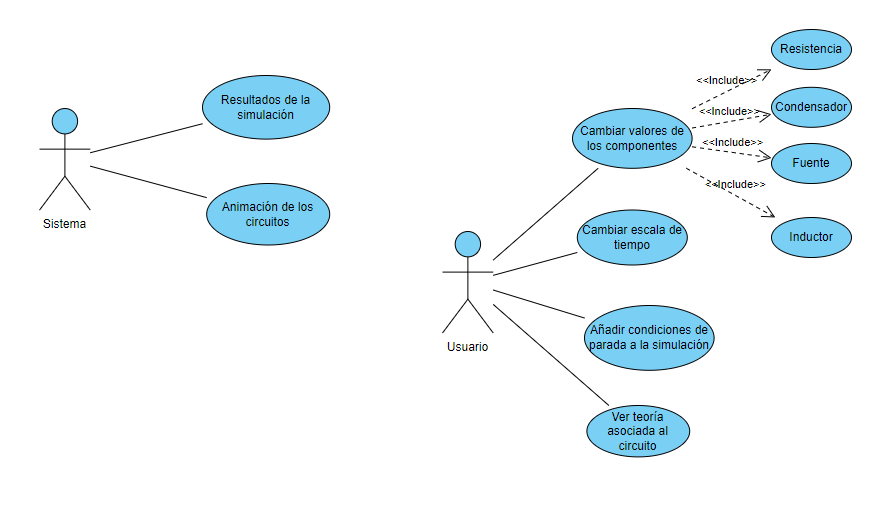
\includegraphics{images/casos_de_uso.PNG}
    \caption{Diagrama de casos de uso}
    \label{fig::casos_de_uso}
\end{figure}

\end{document}